本章では,提案手法について示す.

\section{変形ARマーカの姿勢推定}
提案手法は,円柱に貼り変形したARマーカを機械学習を用いて平面状のARマーカへの復元を行い,
復元を行うときにエンコードされる潜在変数を用いて姿勢推定を行う.
提案手法では,訓練データを円柱に貼られた変形ARマーカに背景テクスチャをつけた図\ref{hennkei}に示す
画像のように用意する.

      \begin{figure}[htbp]
      \begin{center}
      
\includegraphics[width=50mm]{figure/eps/変形.eps}
      \caption{訓練データ.}
      \label{hennkei}
      \end{center}
      \end{figure}

訓練データと同じ姿勢の円柱に貼り付けられた平面状のARマーカ図\ref{heimen}に示す画像のように教師データ
を用意する.提案手法は教師データを使用する教師あり学習を行うオートエンコーダーを用いて
,平面状のARマーカへの復元を行う.

      \begin{figure}[htbp]
      \begin{center}
      
\includegraphics[width=50mm]{figure/eps/平面.eps}
      \caption{教師データ.}
      \label{heimen}
      \end{center}
      \end{figure}

\subsection{学習}
提案手法のオートエンコーダーの学習の流れを図\ref{gakusyu}に示す.
訓練データ図\ref{gakusyu}(b)をオートエンコーダに入力し,出力図\ref{gakusyu}(c)と教師データ図\ref{gakusyu}(a)の損失関数を計算し
差分が小さくなるように学習を行っていく.学習を行うことで変形ARマーカの姿勢を
表現する潜在変数を獲得することができる.
      \begin{figure}[htbp]
      \begin{center}
      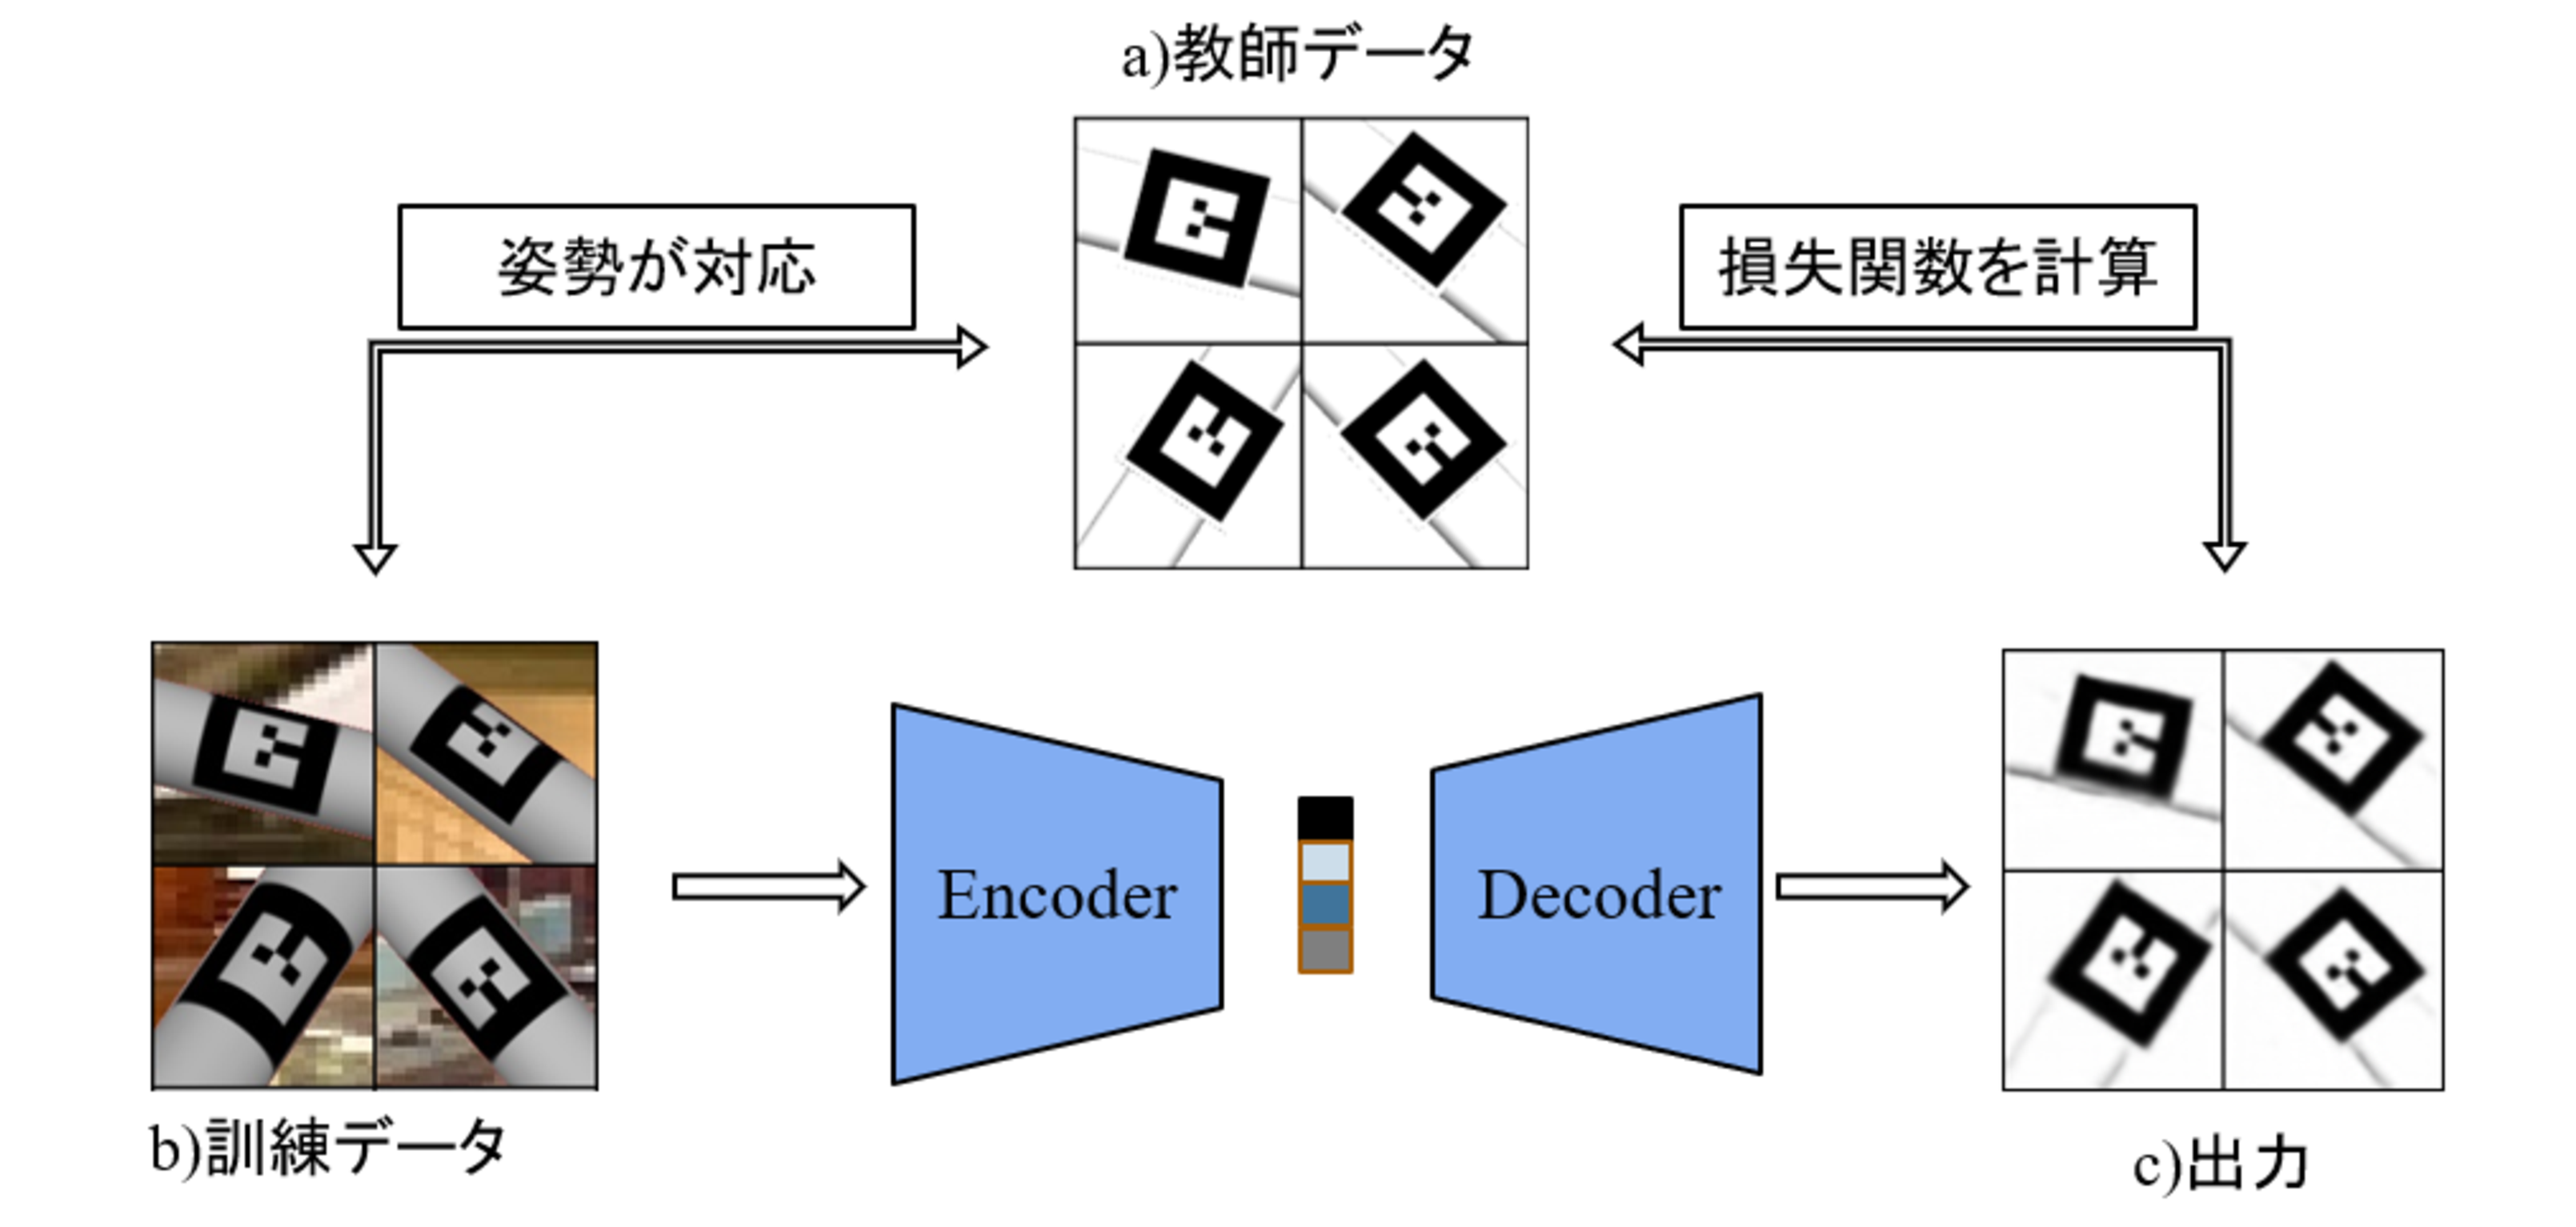
\includegraphics[width=100mm]{figure/eps/提案手法の学習.eps}
      \caption{提案手法の学習の流れ.}
      \label{gakusyu}
      \end{center}
      \end{figure}


\subsection{提案手法による姿勢推定}
姿勢推定を行うためにはデータベースを作成しておく必要がある.データベース作成の流れを図\ref{データベース}に示す.
データベースは,ARマーカの姿勢をrollを0$\sim$360度, pitchを-35$\sim$35度, yawを-15$\sim$15度に範囲を設定し,角度3度刻みで回転させた分解能3度で姿勢画像36,000枚を用意し,エンコーダーに入力する.出力された36,000枚分の潜在変数$z_n$をデータベースとして用意する.

      \begin{figure}[htbp]
      \begin{center}
      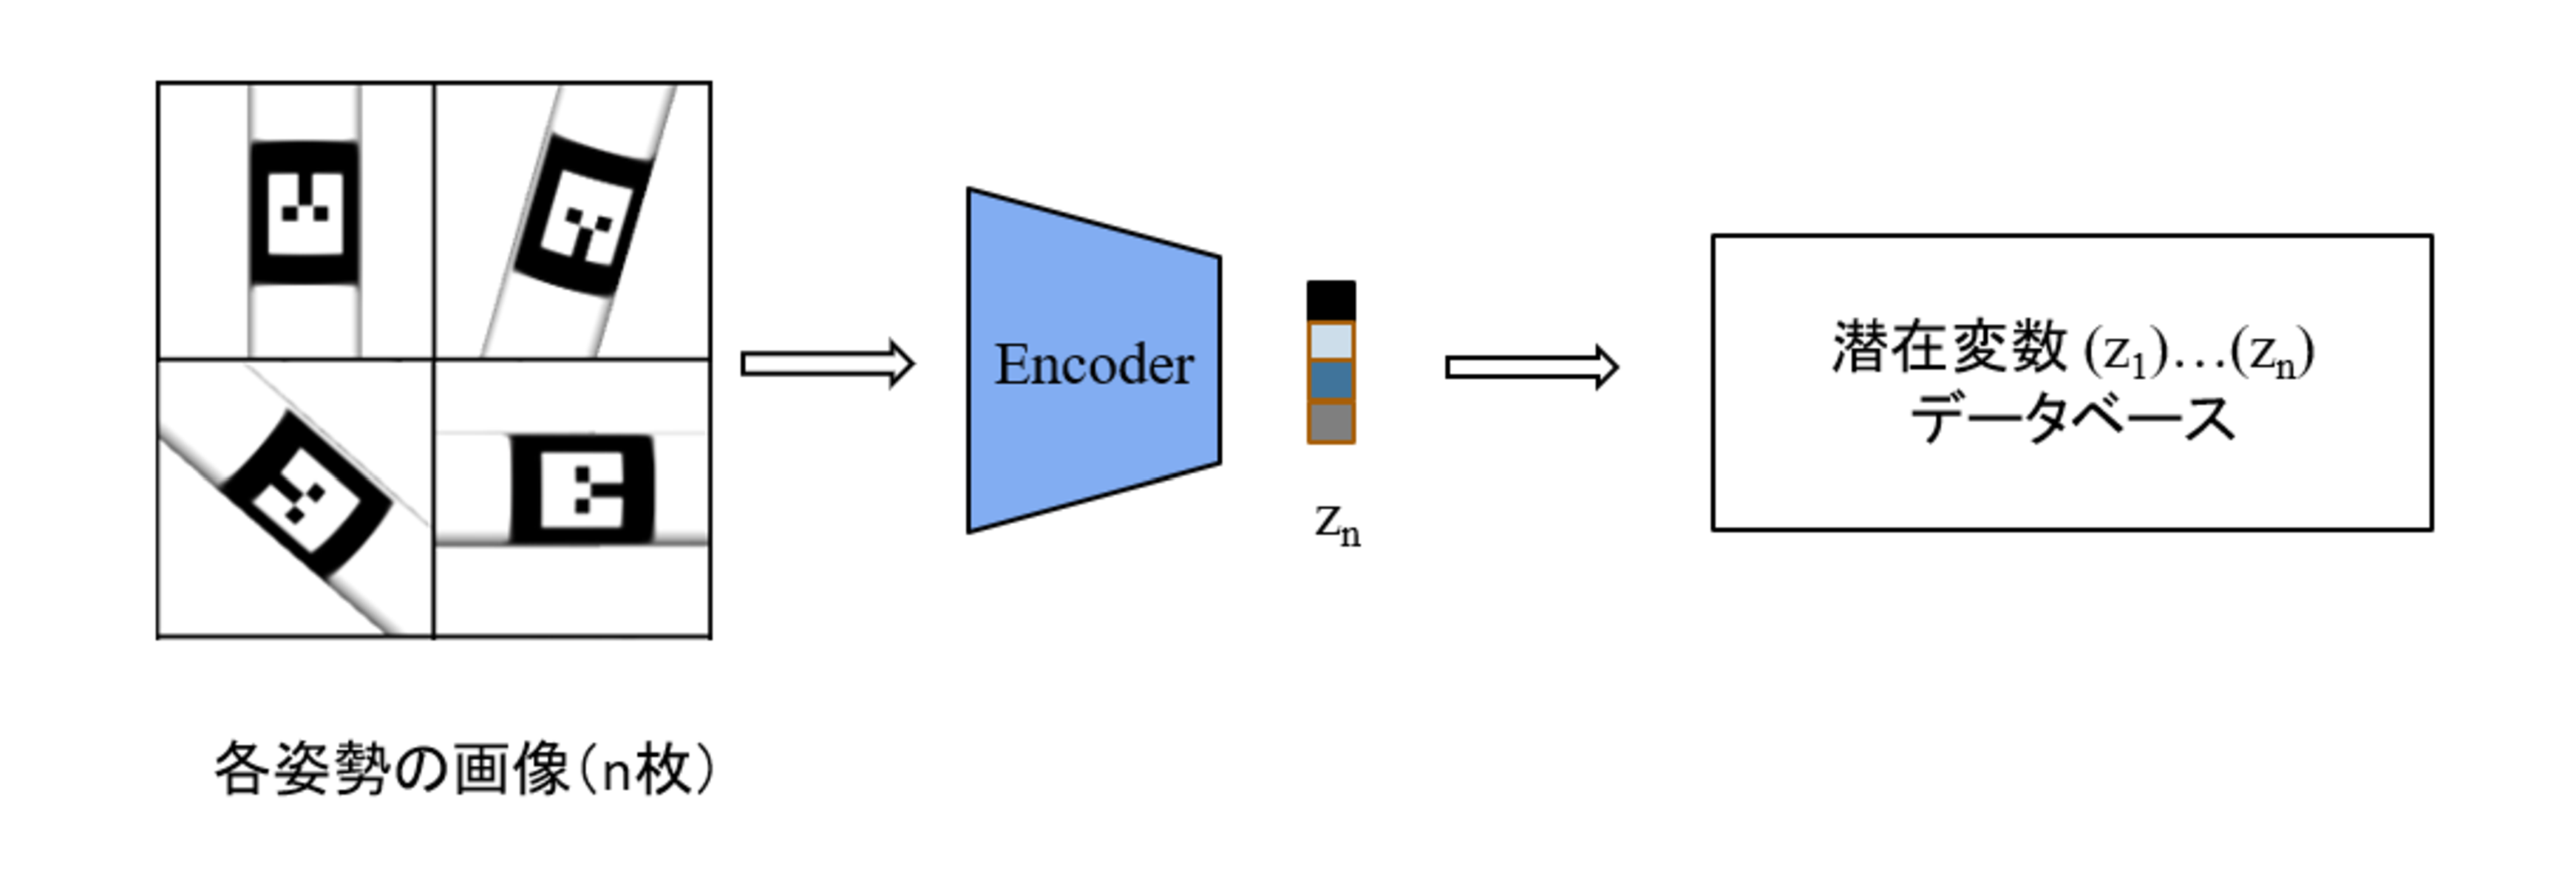
\includegraphics[width=100mm]{figure/eps/データベース.eps}
      \caption{データベースの作成.}
      \label{データベース}
      \end{center}
      \end{figure}

提案手法で行う姿勢推定の流れを図\ref{suitei}に示す.推定対象となる画像を学習済みのオートエンコーダーに入力し潜在変数を取得する.その後,各姿勢の潜在変数を保存したデータベースとの潜在変数をコサイン類似度を用いて最も近い値のデータベースの姿勢を推定姿勢として決定する.

      \begin{figure}[htbp]
      \begin{center}
      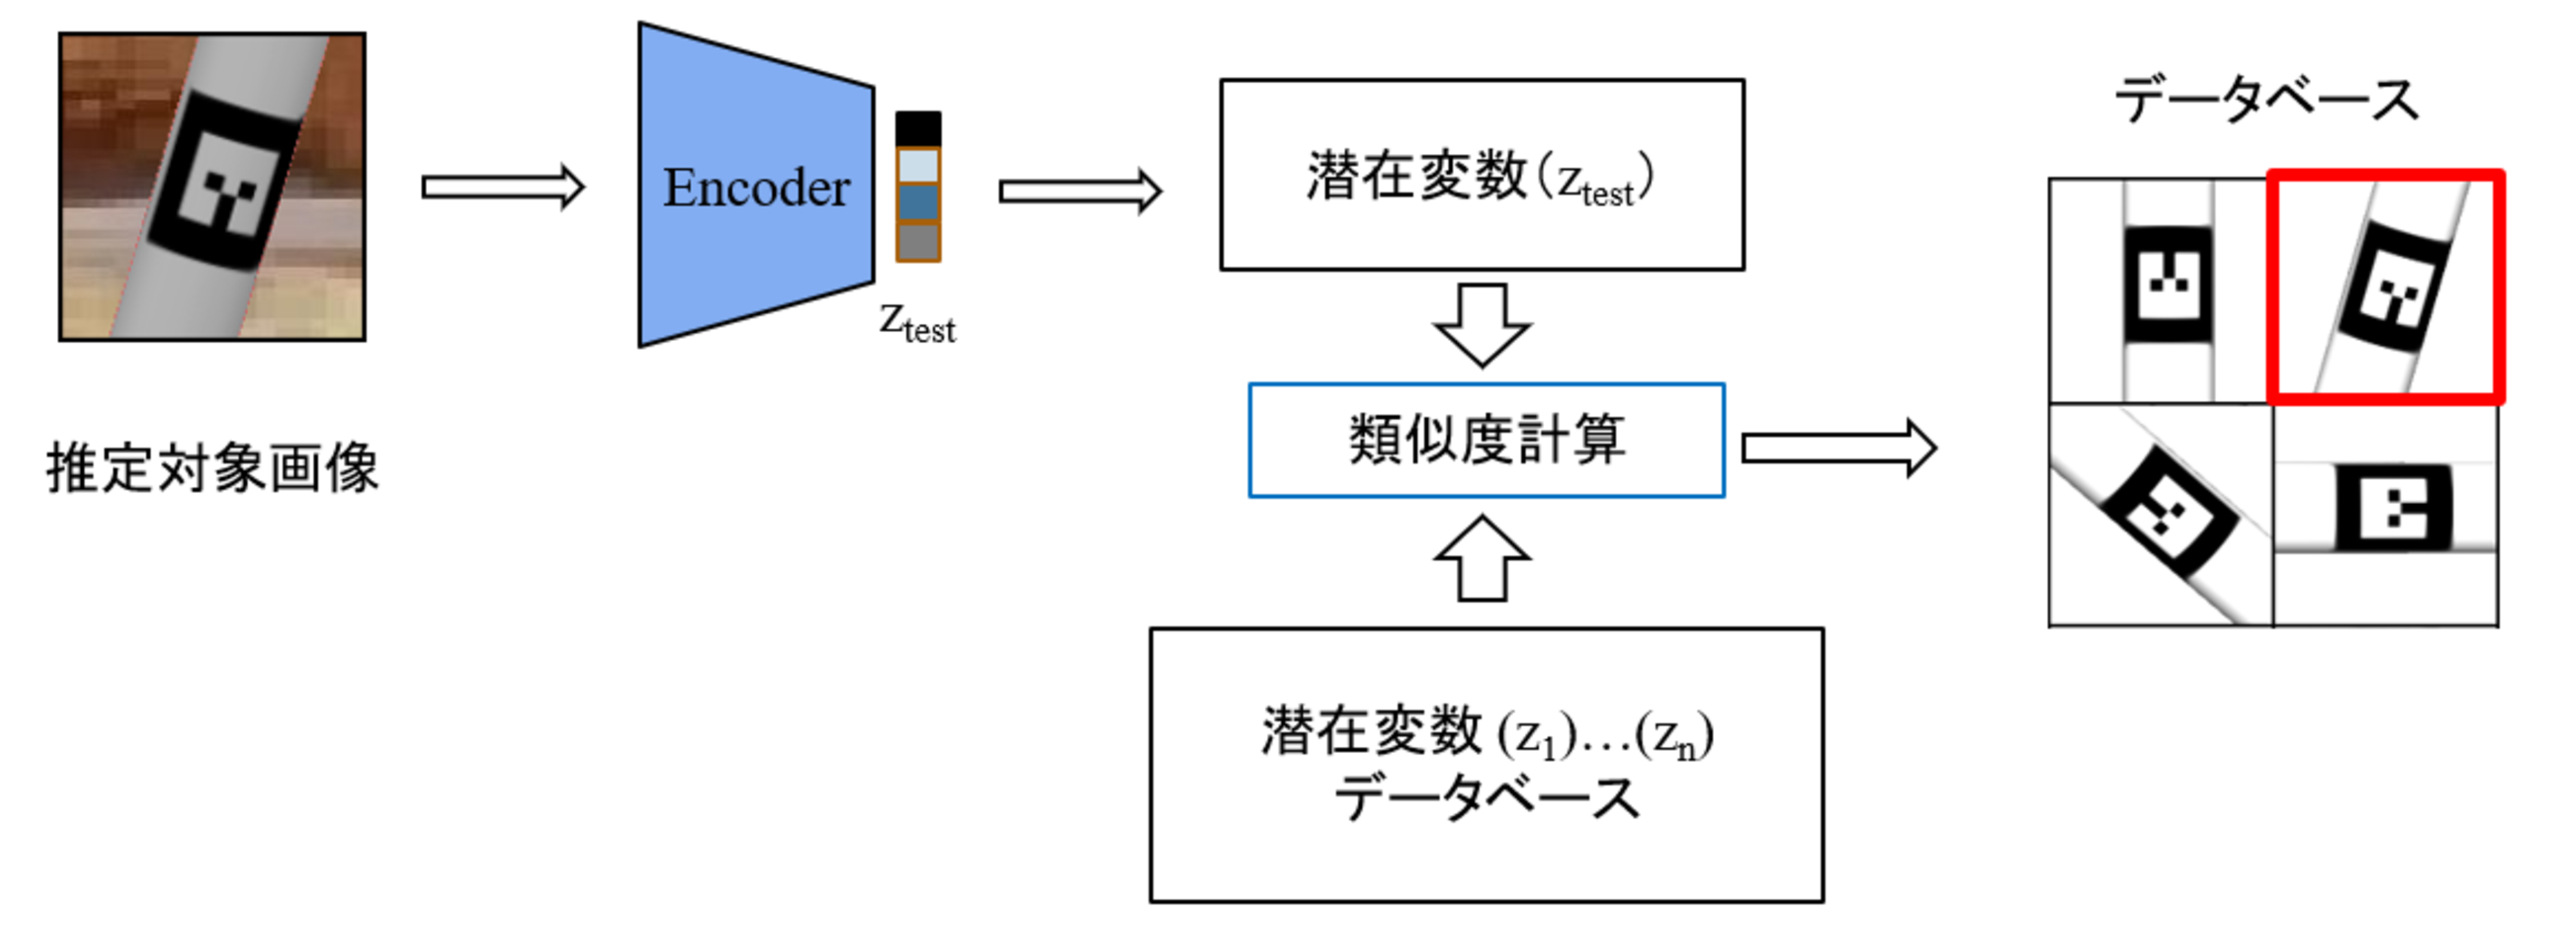
\includegraphics[width=100mm]{figure/eps/提案手法の流れ.eps}
      \caption{提案手法による推定.}
      \label{suitei}
      \end{center}
      \end{figure}

\section{学習データの作成}

提案手法では円柱に沿うように貼られた変形ARマーカモデルと円柱に貼られた平面状のARマーカ図\ref{gazebo2}に示す2つのモデルを使用し学習データを用意する.

      \begin{figure}[htbp]
      \begin{center}
      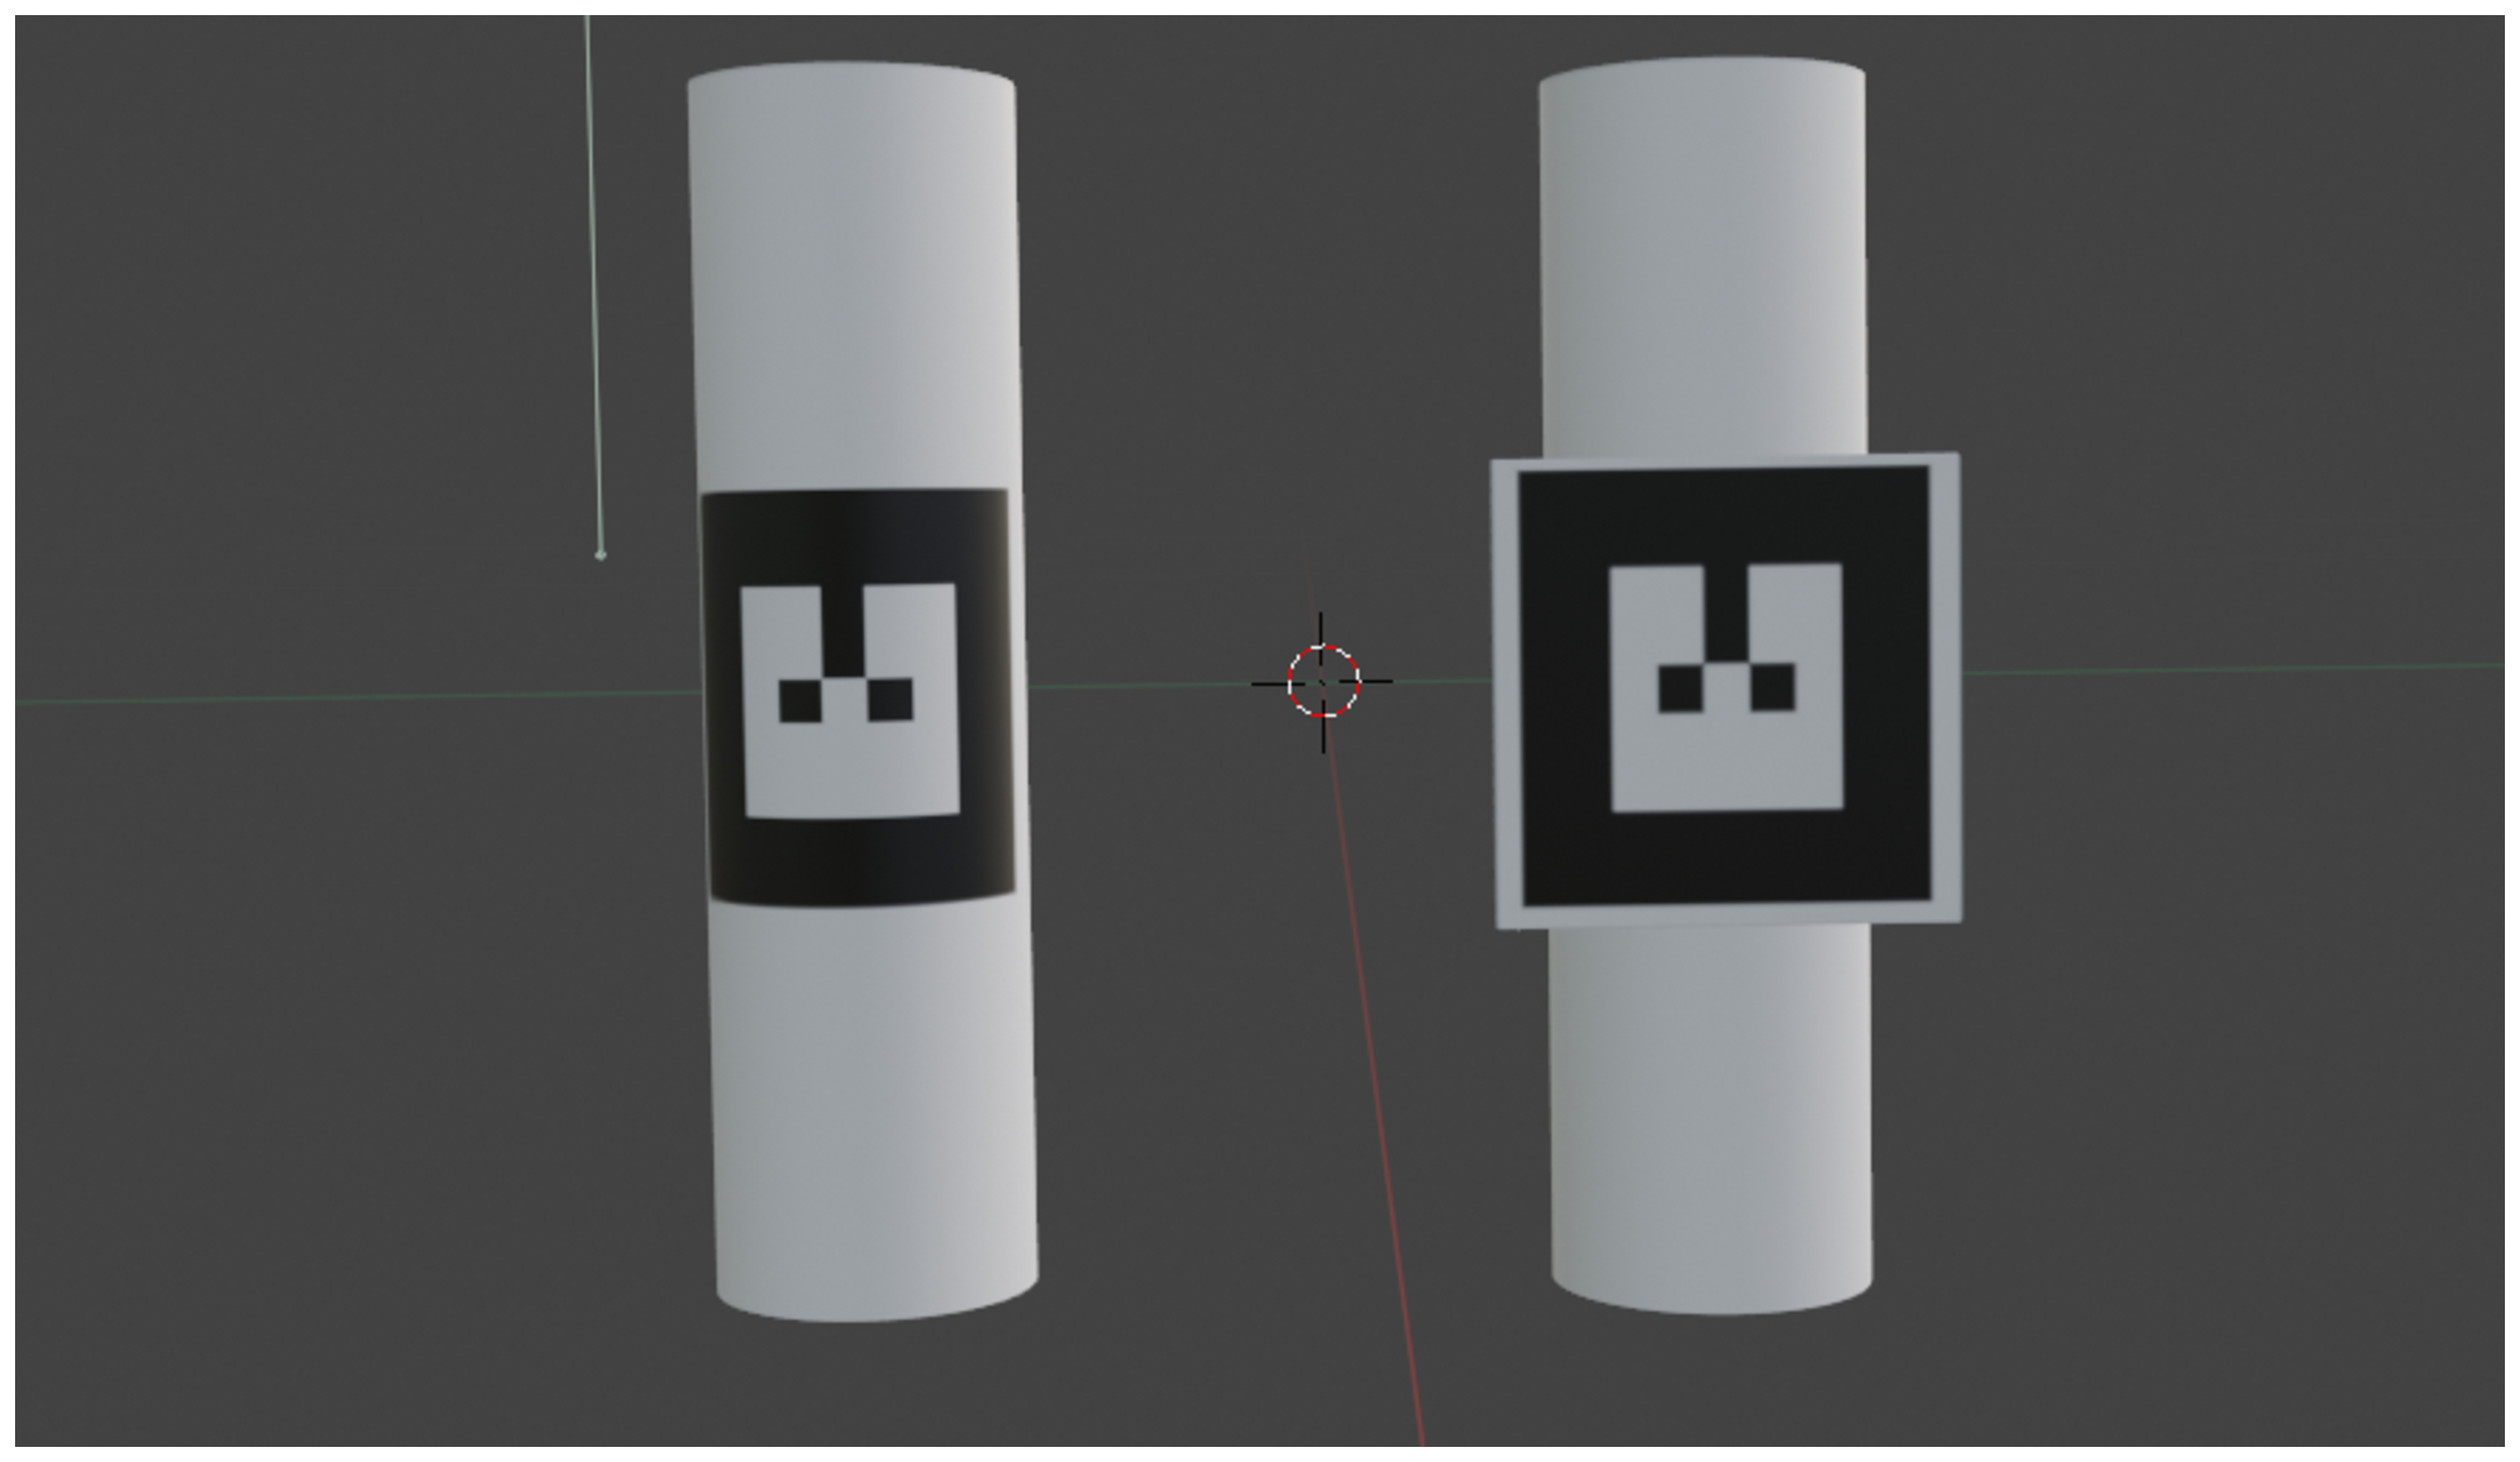
\includegraphics[width=80mm]{figure/eps/二つのモデル.eps}
      \caption{使用するマーカモデル.}
      \label{gazebo2}
      \end{center}
      \end{figure}

\subsection{ARマーカの作成}
ARマーカはROSのパッケージである
ar\_tlack\_alvar
にて用意されている,
マーカID0~9のものを使用する.マーカID0~9を図\ref{09}に示す.

      \begin{figure}[htbp]
      \begin{center}
      \includegraphics[width=80mm]{figure/eps/ARマーカ0~9.eps}
      \caption{使用するARマーカ.}
      \label{09}
      \end{center}
      \end{figure}

ARマーカの大きさはそれぞれ50mmの大きさとなるようにする.
illustratorを用いて変形ARマーカ,平面状ARマーカを円柱モデルに貼り付ける画像を用意する.
平面状のARマーカはblendarを用いて作成する際に50mmの板にARマーカを貼り付け円柱とつなぎ合わせる.
変形ARマーカは直接円柱に貼り付けるため,画素値(255,255,255)の大きさ,縦幅横幅それぞれ作成したい円柱の縦幅と円周に合わせた背景画像にAR マーカが左端中央となるよう貼り画像を作成する.円柱の半径と横幅を表\ref{tab:ARsize}に示す.
\newpage

\begin{table}[h]
  \centering
  \caption{作成するARマーカ画像の大きさ}
    \begin{tabular}{c|c|c} \hline
		半径(mm) & 縦幅(mm) &横幅(mm) \\ \hline \hline
    	20 & 150 & 125.664 \\ \hline
    	30 & 150 & 188.496 \\ \hline
    	40 & 150 & 251.327 \\ \hline
  \end{tabular}
 \label{tab:ARsize}
\end{table}


\subsection{変形ARマーカモデル}

ARマーカを貼り付けた円柱モデルは,blendar\cite{bl}で作成を行う.version2.8を使用する.
blender\cite{bl}を開くと初期状態では立方体が表示されているため削除をする.
図\ref{bl1}に示すように,画面左上の「追加」からメッシュ,cylinderの順番で選択をすると円柱が表示される.


      \begin{figure}[htbp]
      \begin{center}
      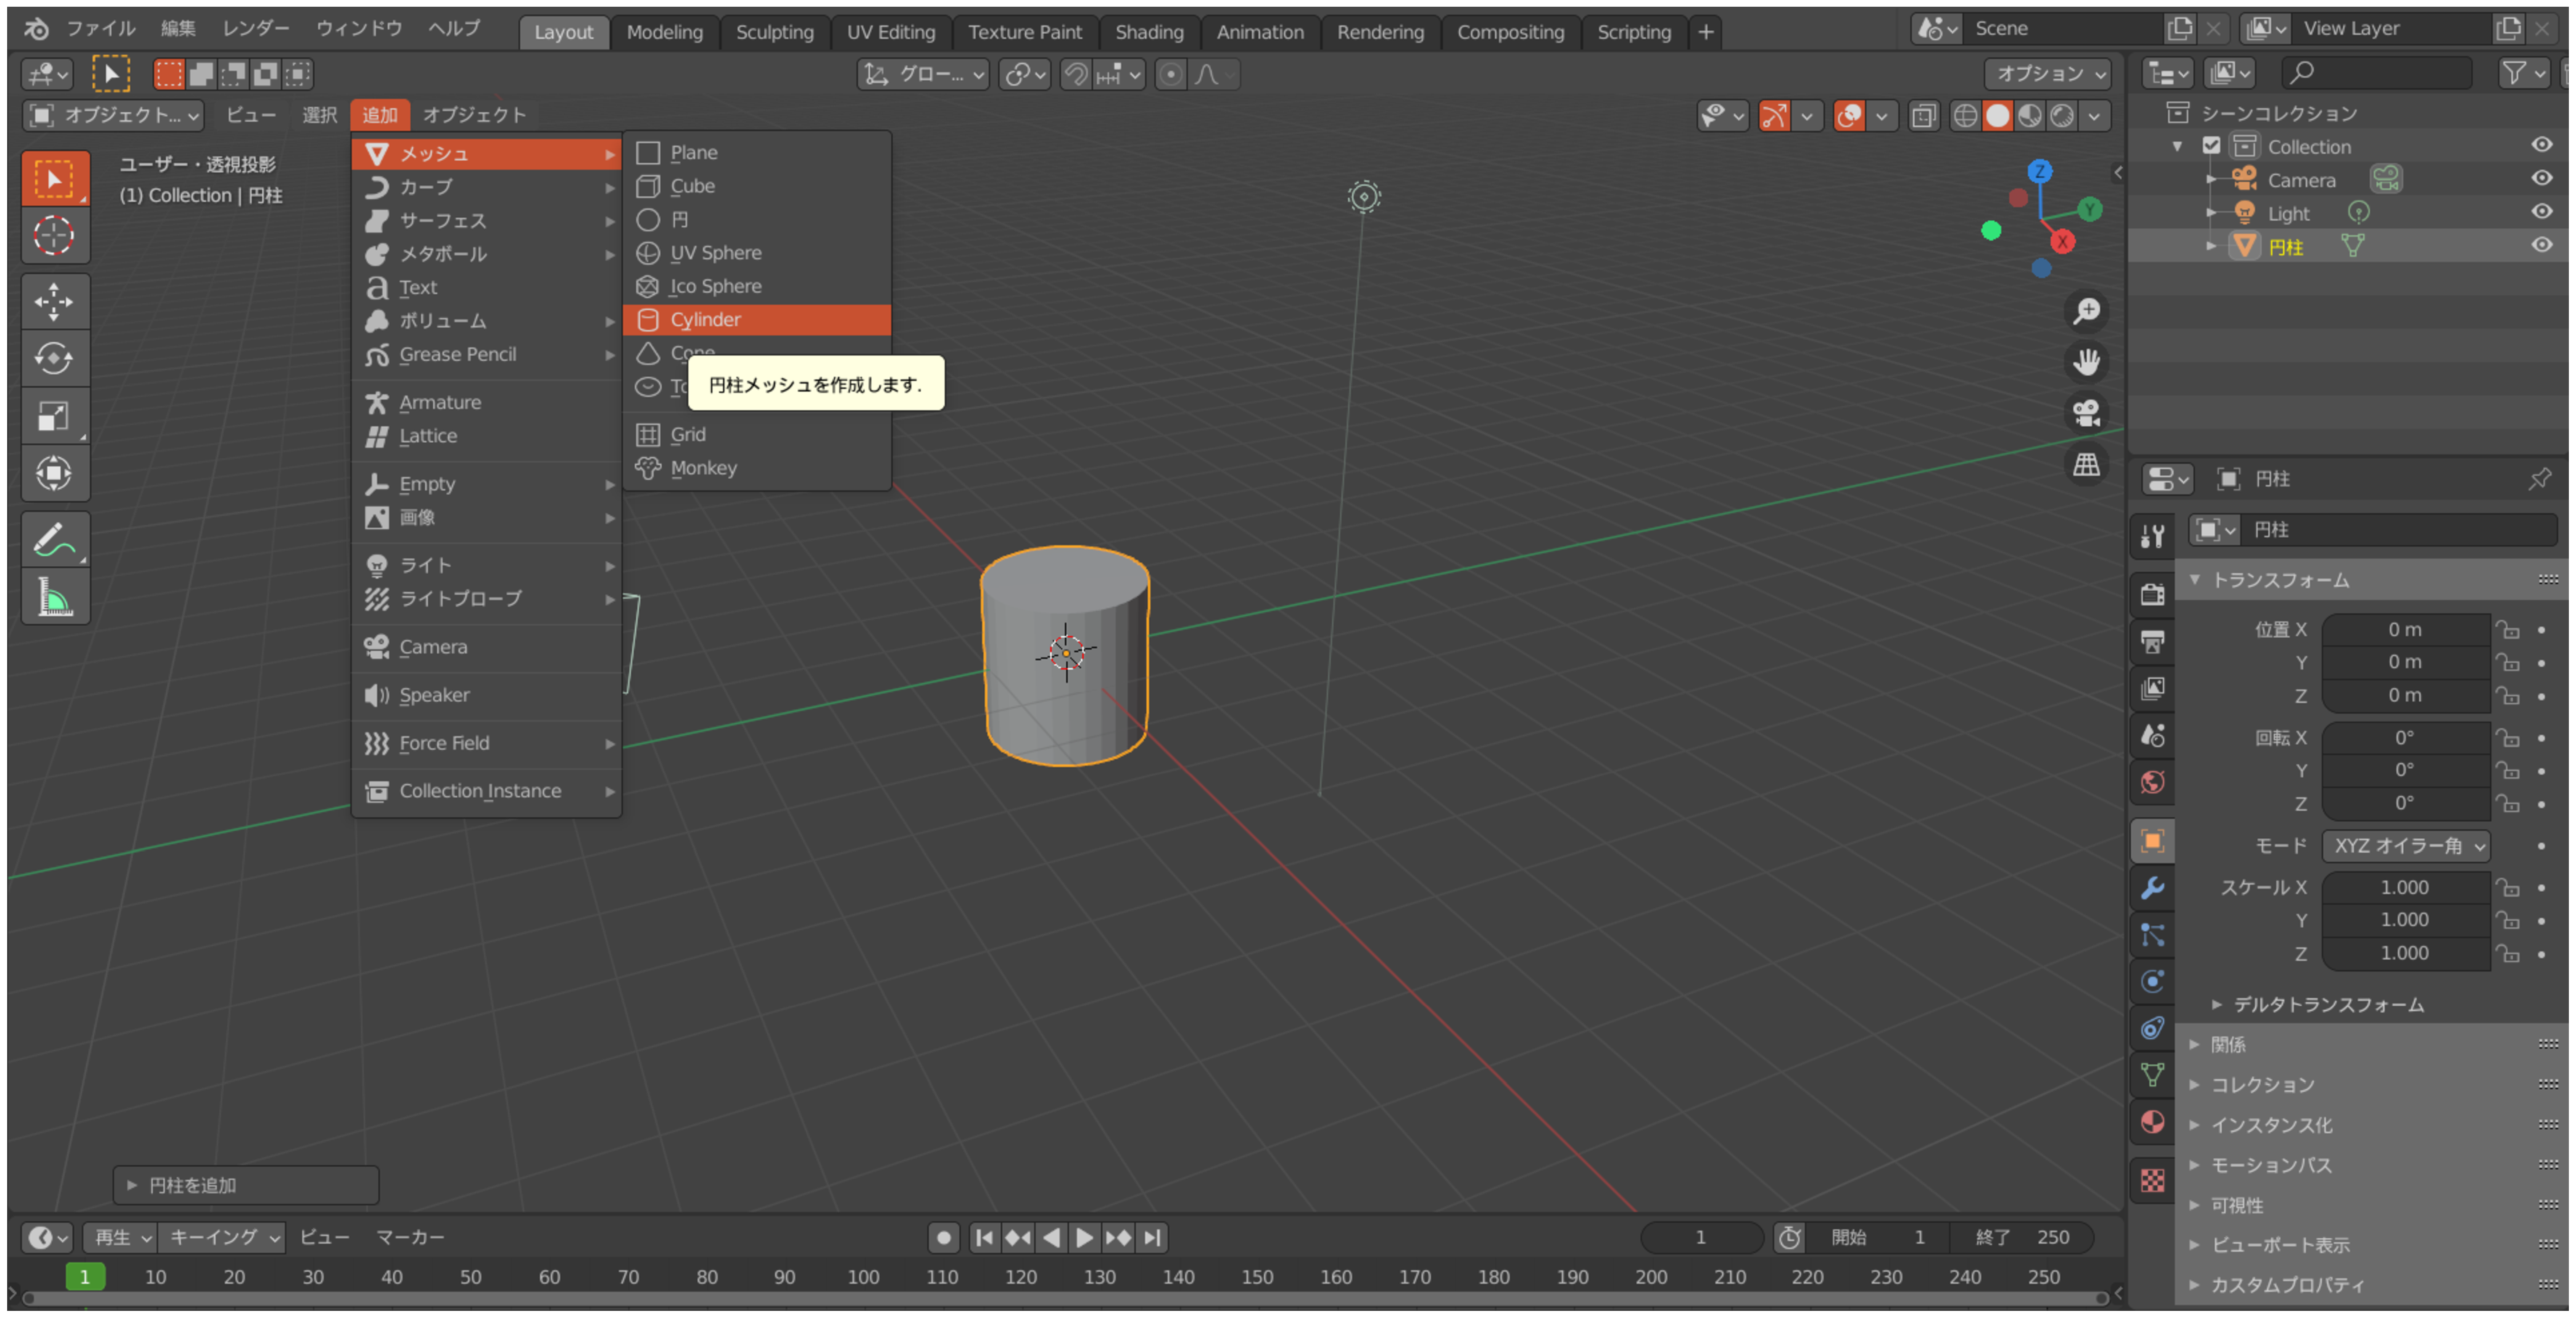
\includegraphics[width=90mm]{figure/eps/bl1.eps}
      \caption{blenderを用いた円柱作成.}
      \label{bl1}
      \end{center}
      \end{figure}




図\ref{bl2}に示すように,左下に表示される「円柱の追加」を選択し,円柱の頂点,半径,深度を変更を行う.
円柱の底面図形は円ではなく正多角形で表現されているため,頂点の数を増やすことで
円に近づける.深度で円柱の縦幅を変えられるため,0.15mに設定する.半径は0.02,0.03,0.04mで用意する.

      \begin{figure}[htbp]
      \begin{center}
      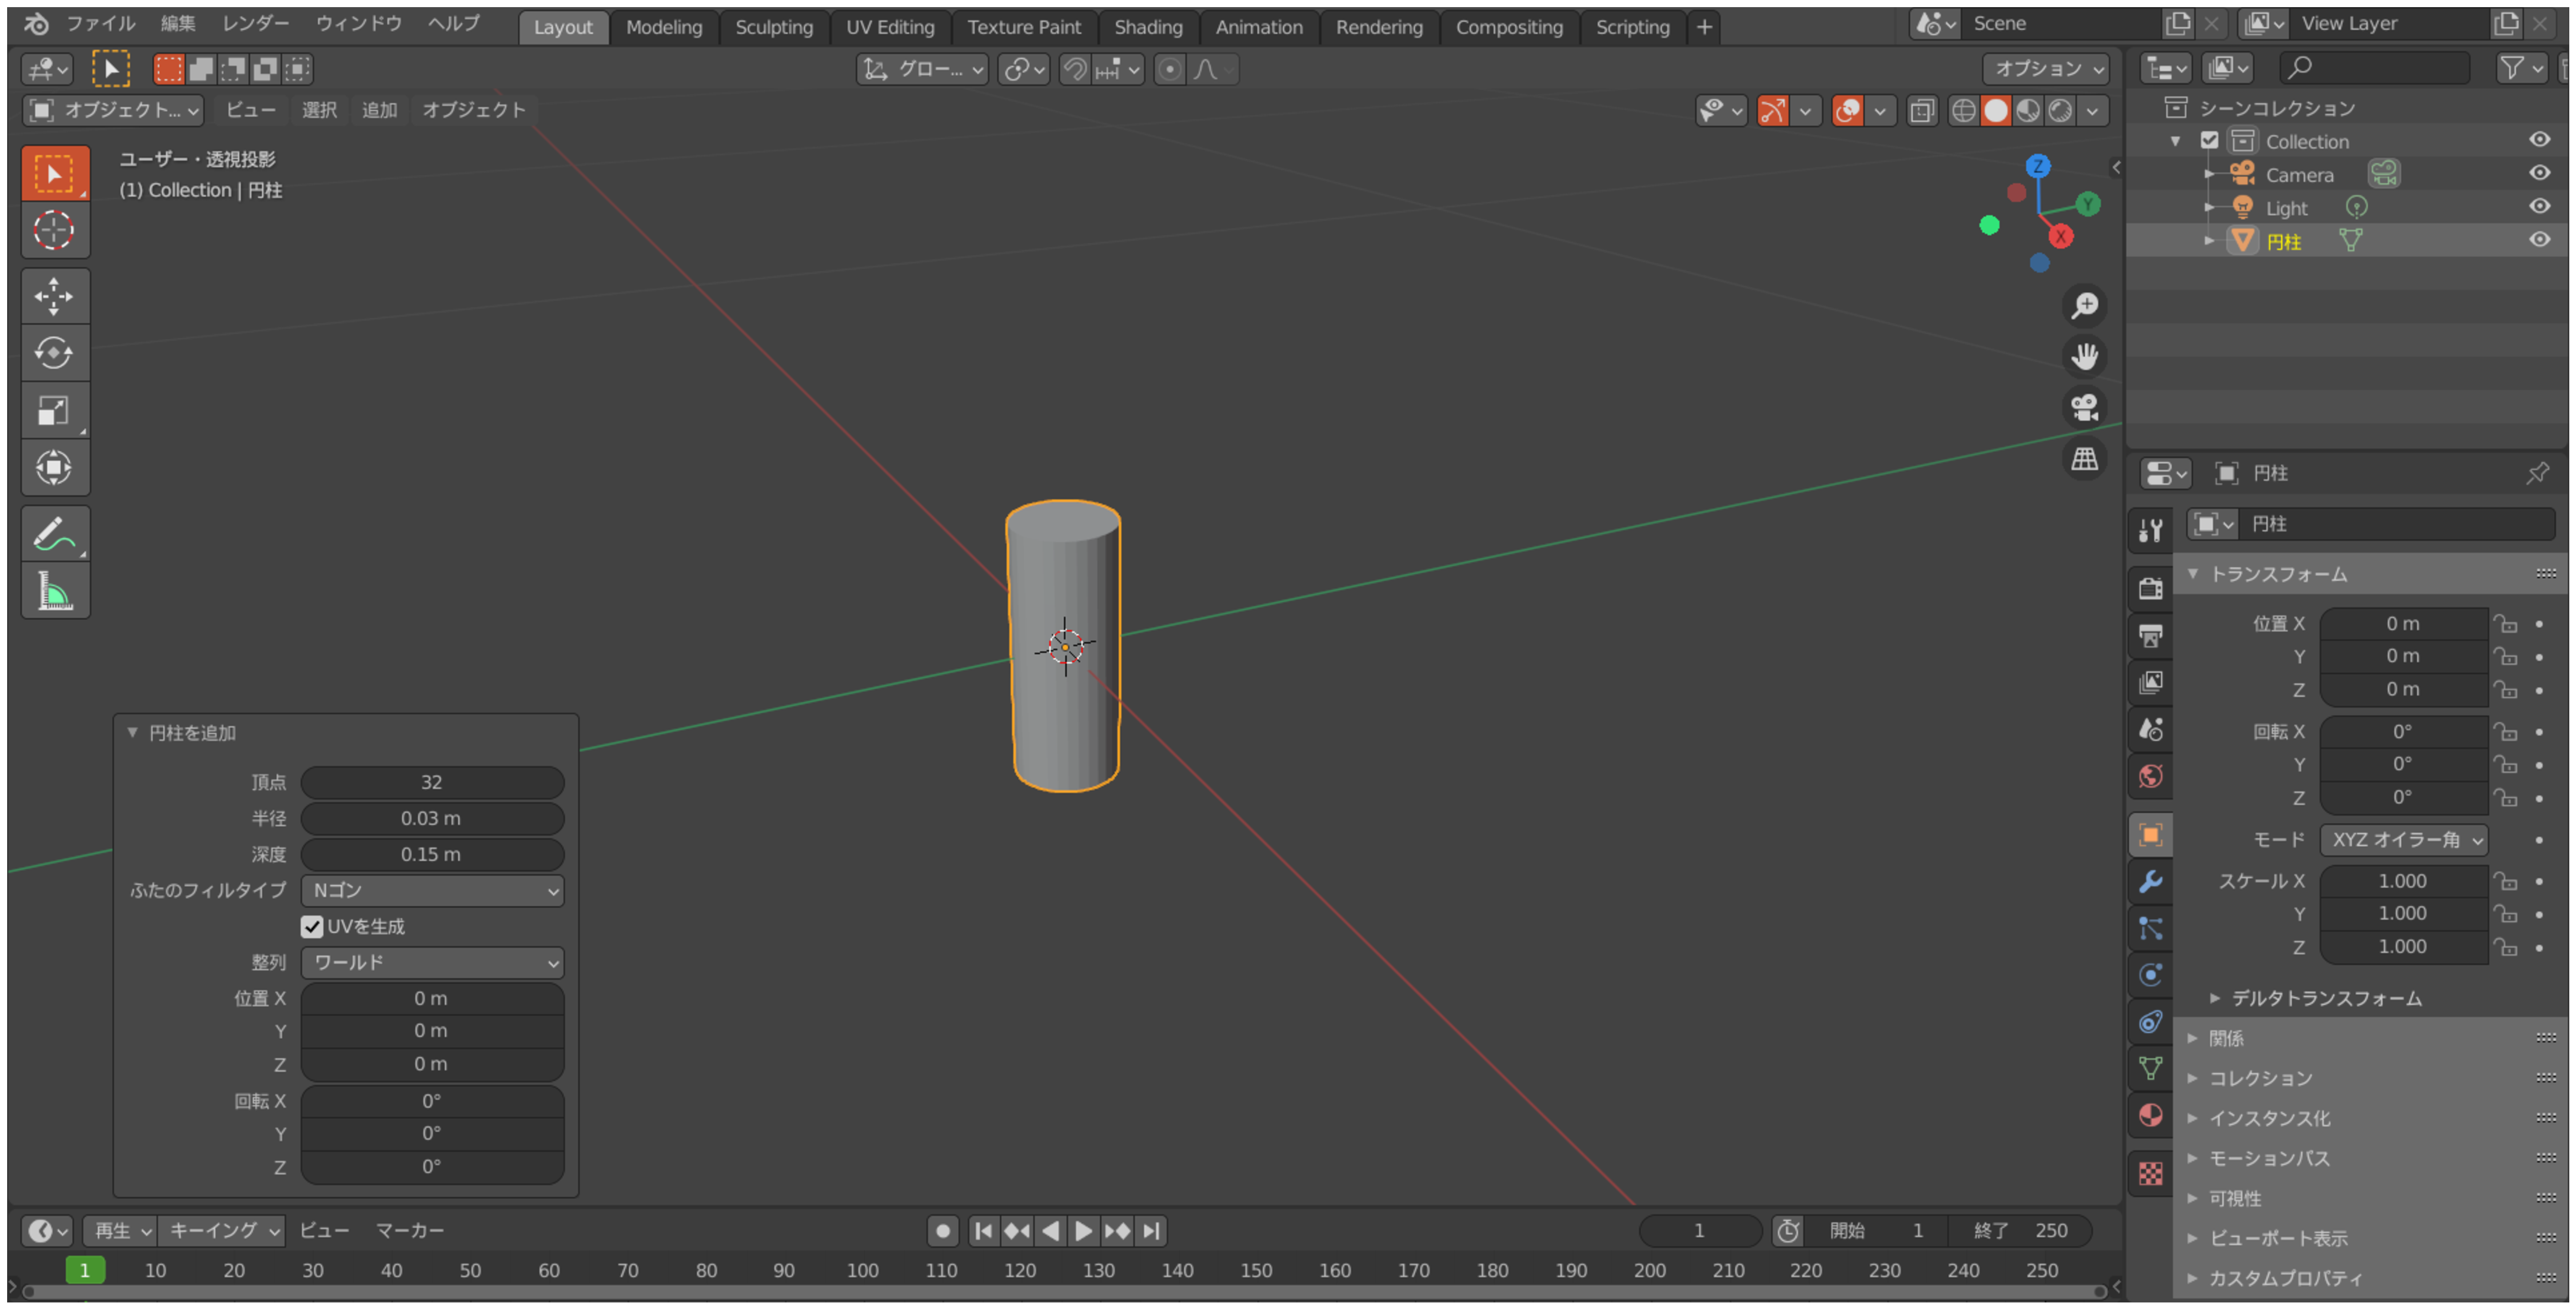
\includegraphics[width=90mm]{figure/eps/bl2.eps}
      \caption{円柱の設定.}
      \label{bl2}
      \end{center}
      \end{figure}

\newpage

画面上部にある「UV Editing」を選択すると画面右側に円柱,左側にマス目が表示される.
編集モードに変更し「面選択」を選択し図\ref{bl3}に示すように底面の削除を行う.

      \begin{figure}[htbp]
      \begin{center}
      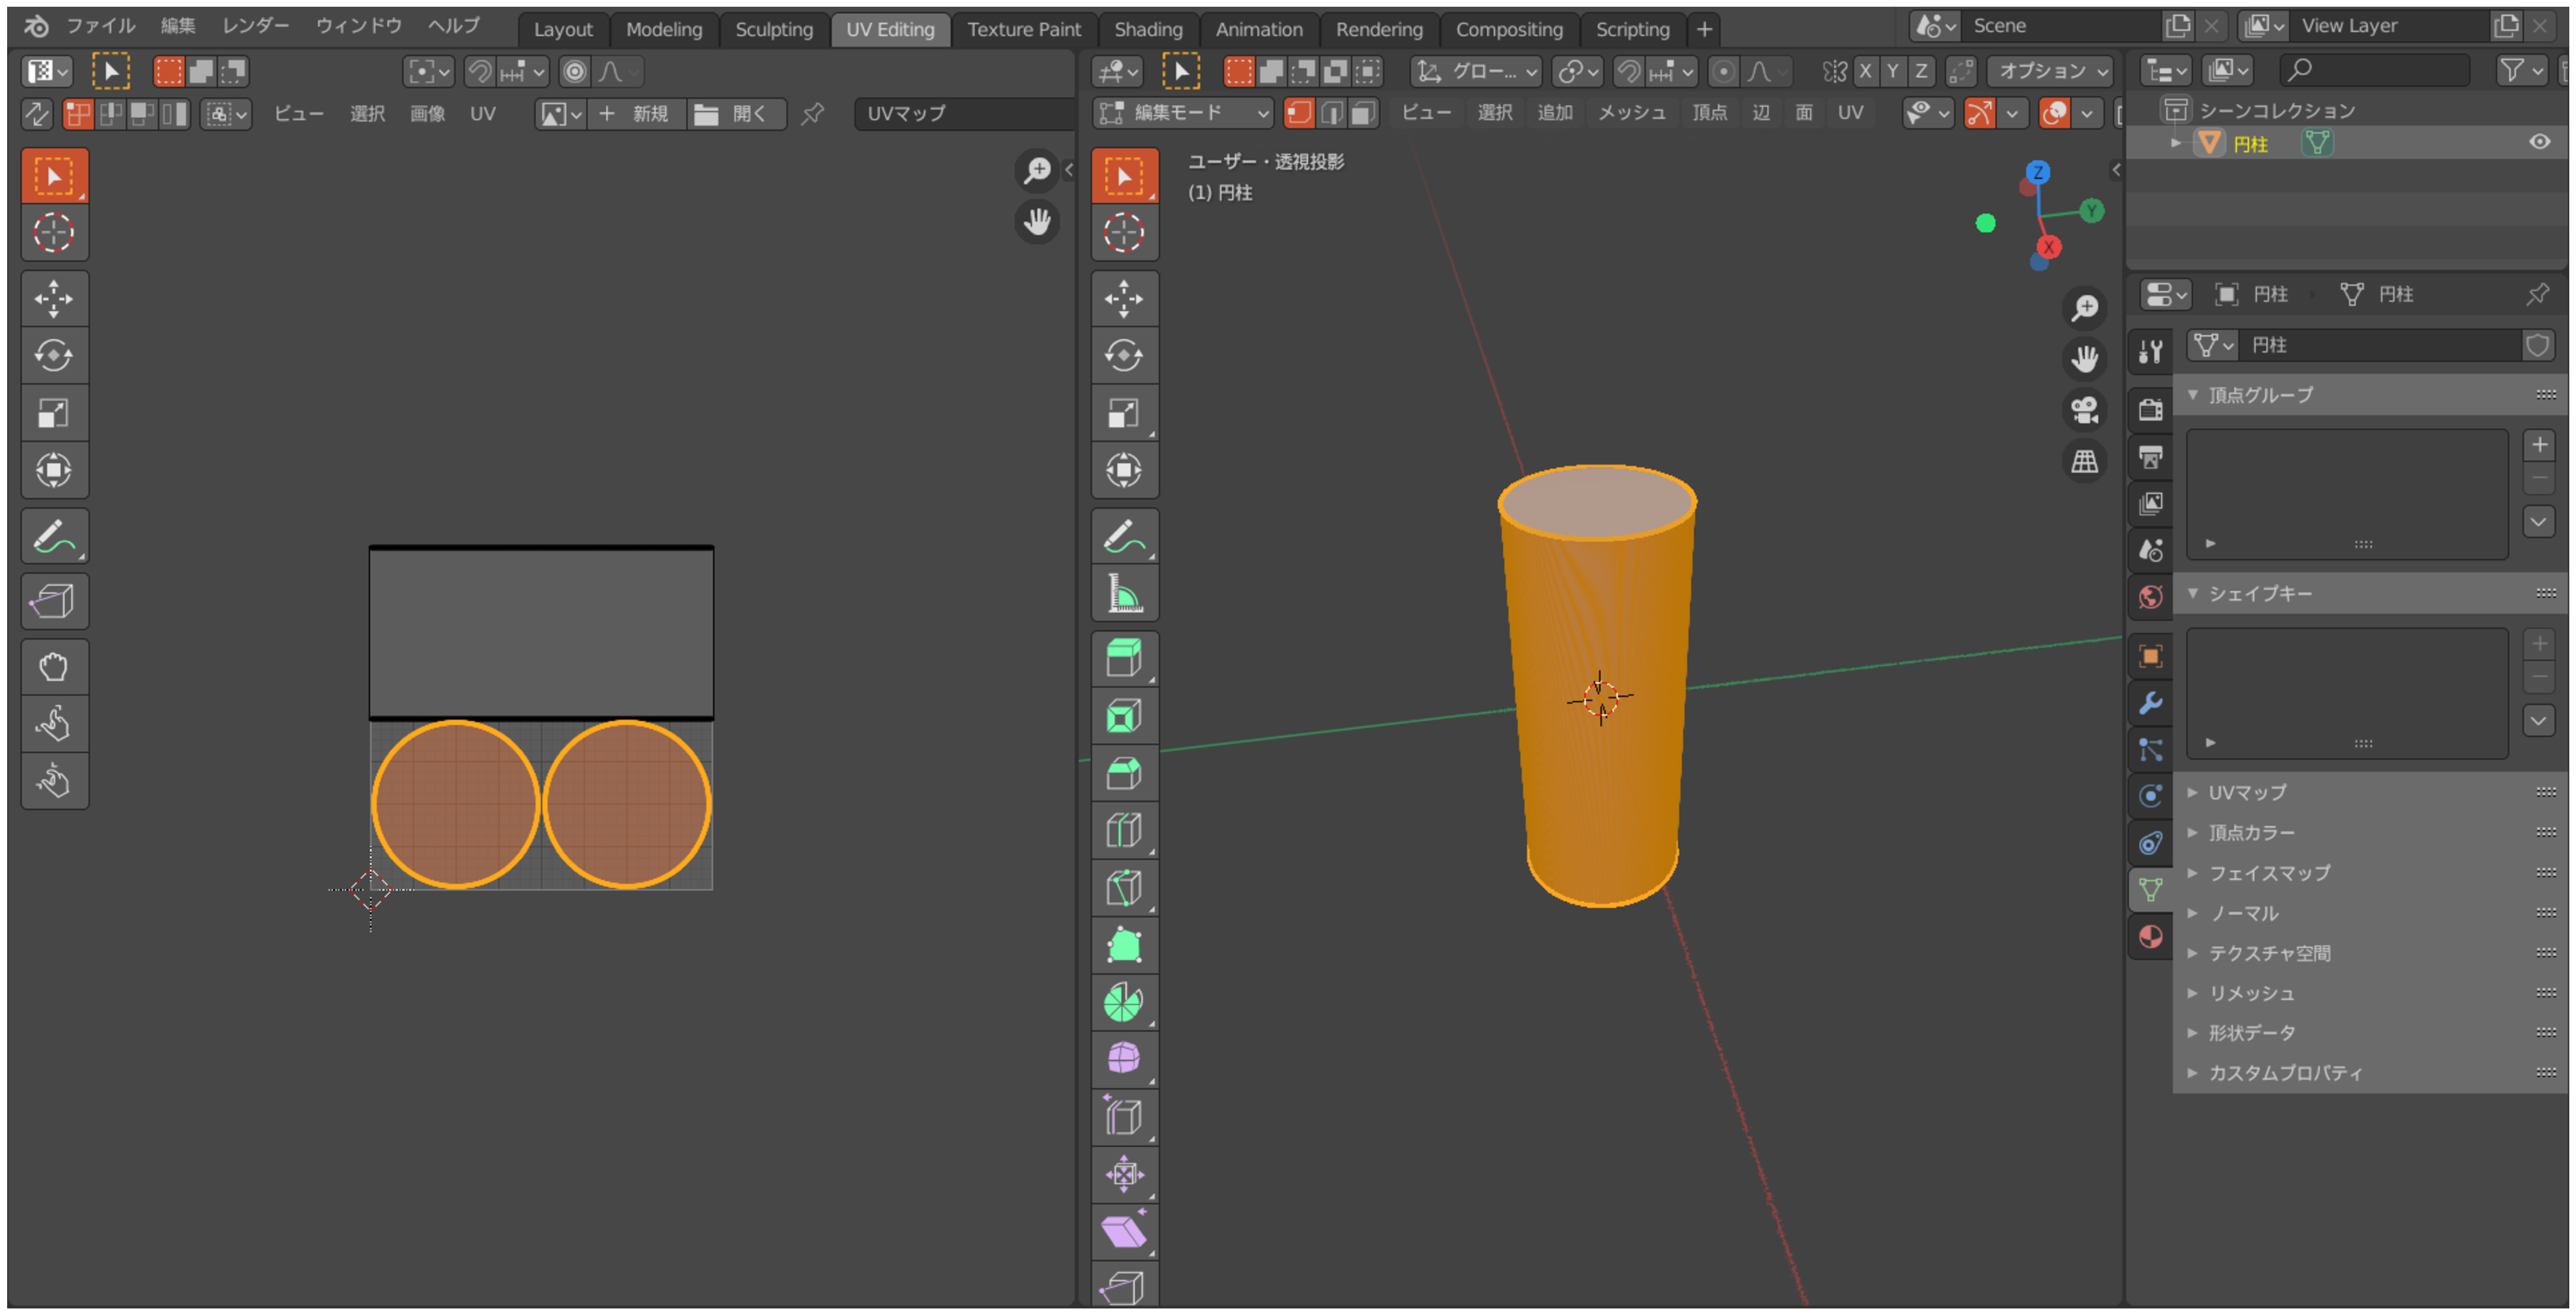
\includegraphics[width=90mm]{figure/eps/bl3.eps}
      \caption{円柱の底面の削除.}
      \label{bl3}
      \end{center}
      \end{figure}




「Modeling」を選択し,画面右下の「Material」を選
択し新規作成を選択,ベースカラーを画像テクスチャにしてから先ほど作成したARマーカ
の画像を開く.右上にあるマテリアルのマークを選択すると図\ref{bl4} のようにAR マーカが貼付
された円柱のモデルができる.


      \begin{figure}[htbp]
      \begin{center}
      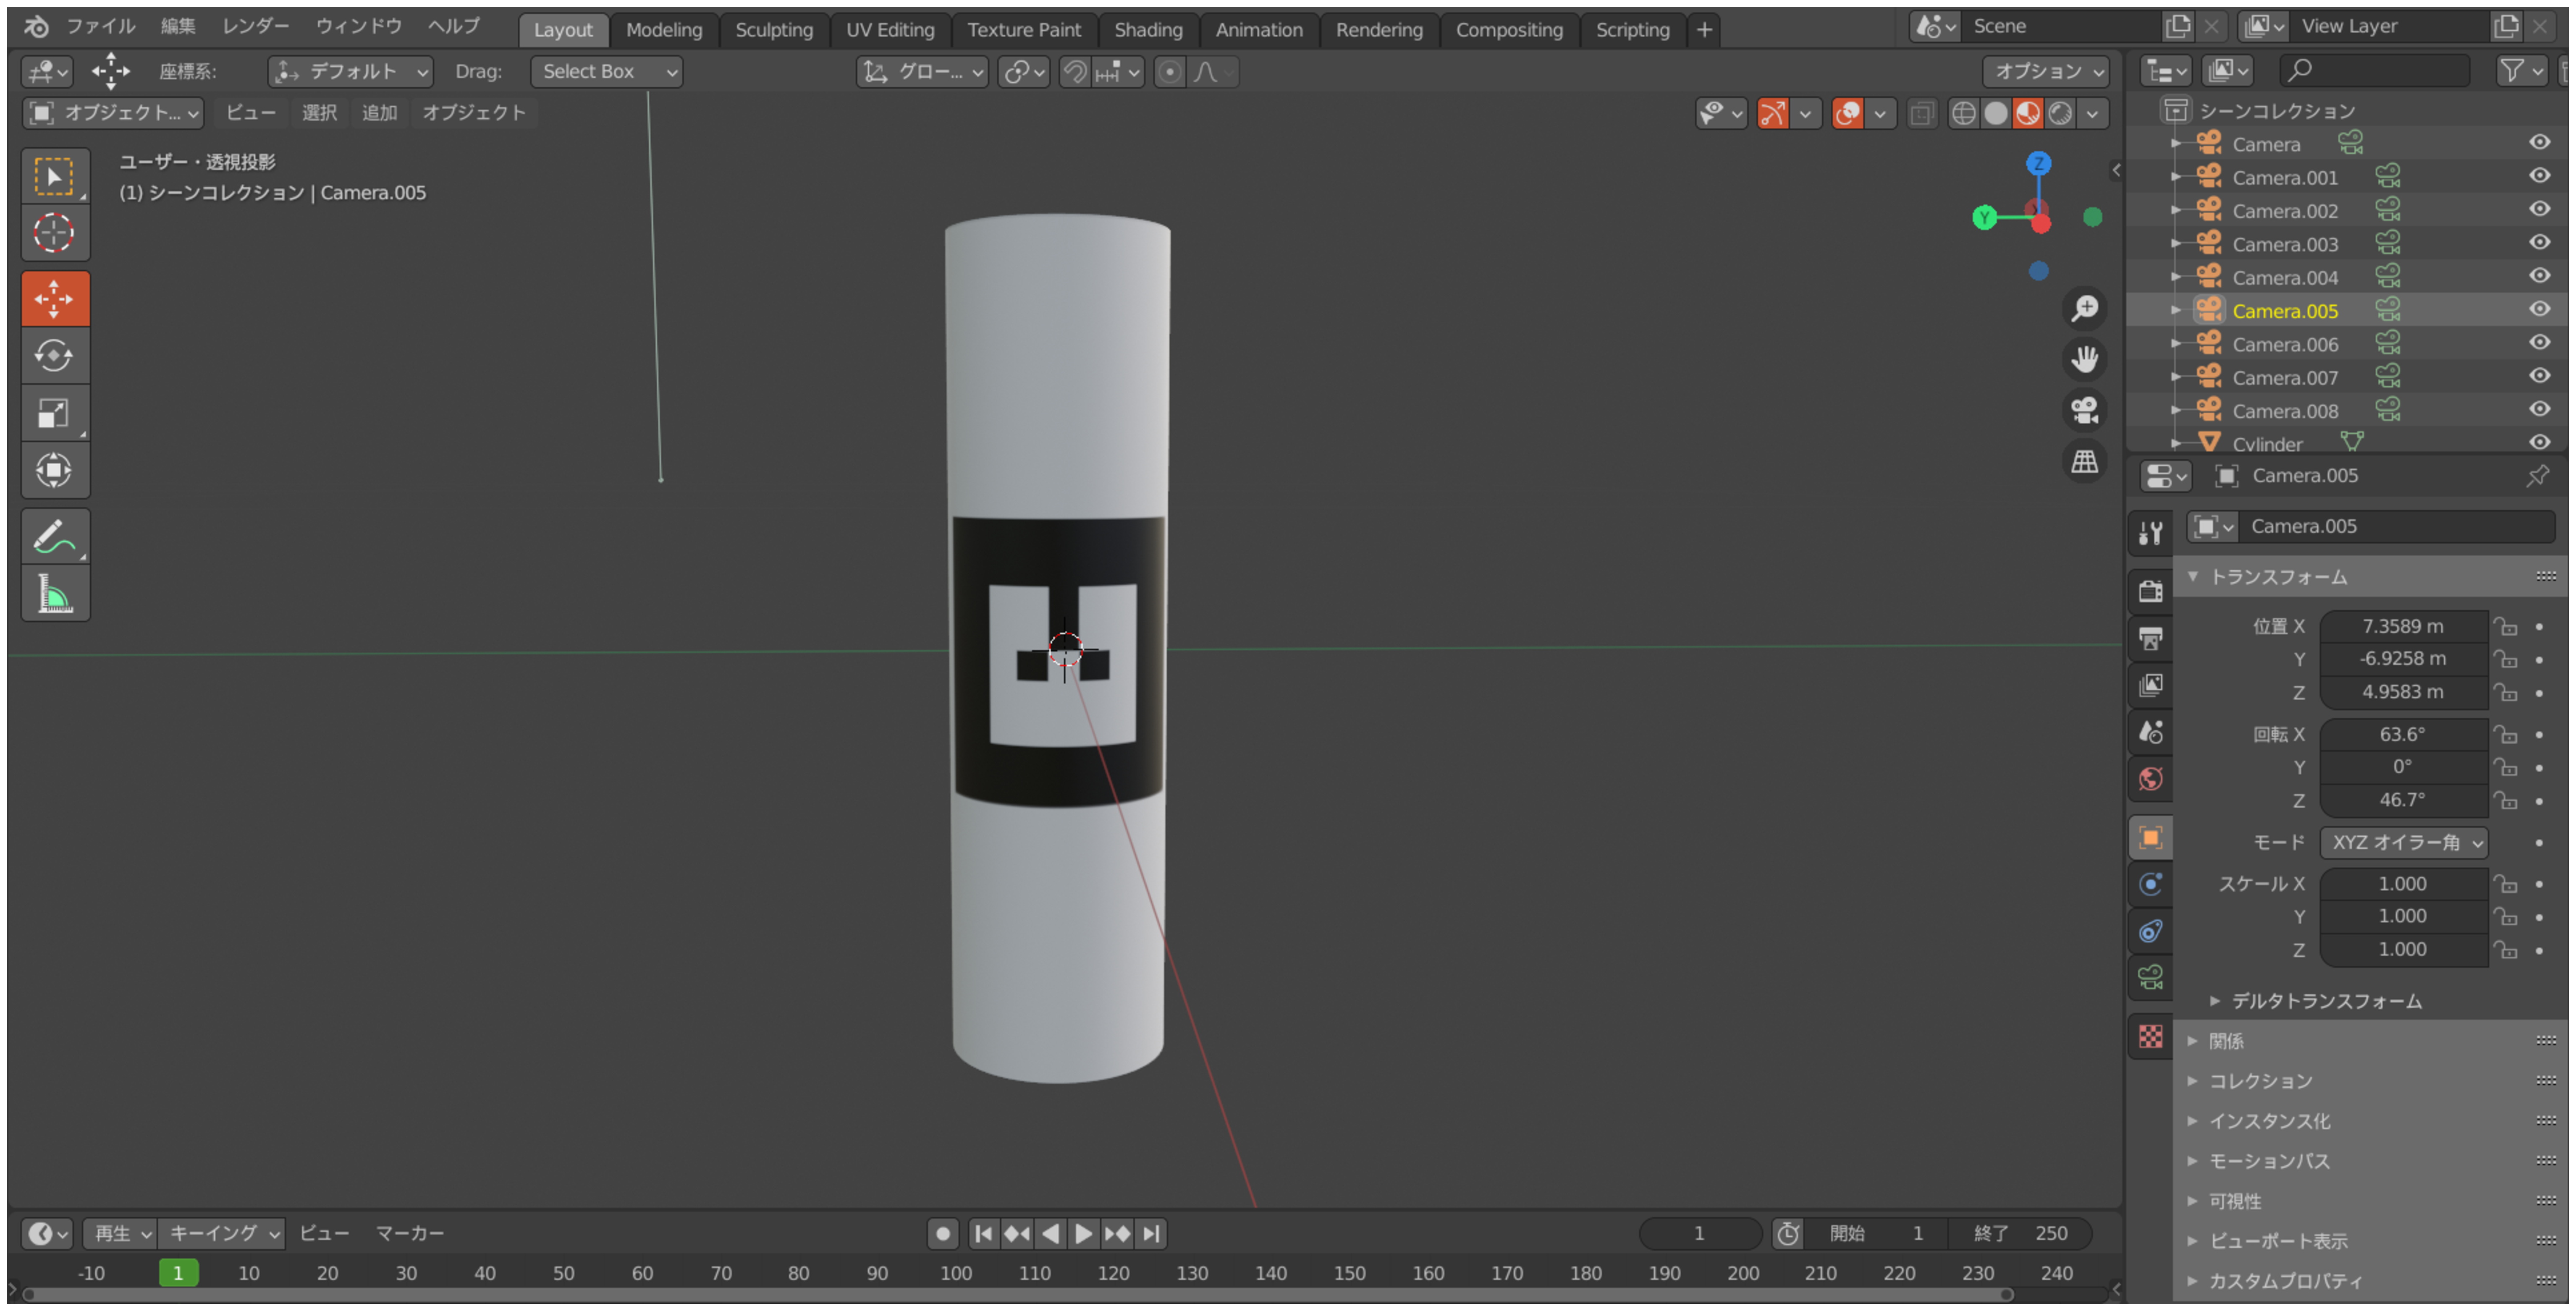
\includegraphics[width=90mm]{figure/eps/bl4.eps}
      \caption{変形ARマーカの完成図.}
      \label{bl4}
      \end{center}
      \end{figure}



この手順で,円柱に貼られたマーカを半径3種類とID10種類の合計30種類のモデルを作成する.また,平面状ARマーカの30種類も同様の手順で板にマーカを張り付け円柱と結合を行い作成する.




\subsection{学習用画像の撮影}
学習用画像は,変形ARマーカモデルと平面状ARマーカモデルをgazebo\cite{ga}の環境を用いて撮影を行う.
カメラは座標(0,0,0.5)の位置に設置し,画像サイズ(1920$\times$1080)で撮影を行う.
モデルの背景には,変形ARマーカは後で背景画像を合成できるように赤色の板を設置,平面状ARマーカの背景には白色の板を設置する.このままの環境では暗いためuser\_point\_lightを座標位置(x,y,z)がそれぞれ(1,1,1.2),(1,1,0.8),(0,0,1.2),(0,0,0.8),(1,-1,1.2),(1,-1,0.8)で配置を行い,壁が均一な明るさとなるよう撮影する.

変形AR マーカと平面状ARマーカのIDと半径が同じ種類をセットとなるように.それぞれ別のファイルに姿勢と名前が同じとなるように保存していく.変形ARマーカは(0,0,0.015)の位置を中心に(x,y,z)が最小値(0.3,-0.24,0.35)から最大値(0.8,0.24,0.65)の範囲に出現するように設定し,平面状ARマーカは(x,y,z)が(0.8,0,0.5)の位置に配置する.
ARマーカの姿勢はマーカが半分以上見える回転範囲[roll0~360°,pitch-35~35°,yaw-15~15°]に設定して撮影を行う.
撮影後,変形ARマーカの背景にテクスチャの合成を行う.
それぞれの画像をARマーカが写る位置でトリミングを行い,128$\times$128にリサイズをする.学習用に用意した同じ姿勢の変形ARマーカと平面状ARマーカの画像を図\ref{hennkei}図\ref{heimen}に示す.1種類あたり,1500枚ずつ用意する.訓練データ教師データ合わせて60種類$\times$1500枚の合計90000枚の画像を用意する.















